\title{\vspace{-5ex} \large Project 1 :: Defeating SkyNet \\ \large (Security Essentials)\vspace{-2ex}}
\author{\large Dean Pisani 311210775 \\ \large Kristy Hughes 310186293\vspace{-2ex}}
\date{}

\documentclass[9pt,a4paper]{article}
\usepackage{geometry}
\usepackage{listings}
\usepackage{color}
\usepackage{setspace}
\usepackage{amsmath}
\usepackage{sectsty}
\usepackage{graphicx}

\sectionfont{\fontsize{11}{9}\selectfont}

% Set up python syntax highlighting
\definecolor{Code}{rgb}{0,0,0}
\definecolor{Decorators}{rgb}{0.5,0.5,0.5}
\definecolor{Numbers}{rgb}{0.5,0,0}
\definecolor{MatchingBrackets}{rgb}{0.25,0.5,0.5}
\definecolor{Keywords}{rgb}{0,0,1}
\definecolor{self}{rgb}{0,0,0}
\definecolor{Strings}{rgb}{0,0.63,0}
\definecolor{Comments}{rgb}{0,0.63,0.2}
\definecolor{Backquotes}{rgb}{0,0,0}
\definecolor{Classname}{rgb}{0,0,0}
\definecolor{FunctionName}{rgb}{0,0,0}
\definecolor{Operators}{rgb}{0,0,0}
\definecolor{Background}{rgb}{0.98,0.98,0.98}

\lstnewenvironment{python}[1][]{
\lstset{
numbers=left,
numberstyle=\footnotesize,
numbersep=1em,
xleftmargin=1em,
framextopmargin=2em,
framexbottommargin=2em,
showspaces=false,
showtabs=false,
showstringspaces=false,
frame=l,
tabsize=4,
% Basic
basicstyle=\ttfamily\small\setstretch{1},
backgroundcolor=\color{Background},
language=Python,
% Comments
commentstyle=\color{Comments}\slshape,
% Strings
stringstyle=\color{Strings},
morecomment=[s][\color{Strings}]{"""}{"""},
morecomment=[s][\color{Strings}]{'''}{'''},
% keywords
morekeywords={import,from,class,def,for,while,if,is,in,elif,else,not,and,or,print,break,continue,return,True,False,None,access,as,,del,except,exec,finally,global,import,lambda,pass,print,raise,try,assert},
keywordstyle={\color{Keywords}\bfseries},
% additional keywords
morekeywords={[2]@invariant},
keywordstyle={[2]\color{Decorators}\slshape},
emph={self},
emphstyle={\color{self}\slshape},
%
}}{}

\begin{document}
\maketitle
\small
\setlength{\parindent}{0pt}

\section{Low Level Exploits}

\subsection{Savegames}
\begin{enumerate}
\item A buffer overflow can be executed by typing a name longer than 10 bytes.\\
E.g.\\
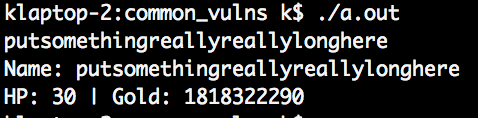
\includegraphics[scale=0.6]{overflow}

\item For C code in general, the advice to avoid buffer overflows is:
\begin{itemize}
\item Making sure that memory auditing is done properly with valgrind
\item using fgets instead of gets
\item use strncmp() instead of strcmp() or strncpy() instead of strcpy() etc
\end{itemize}

In the case of savegame.c, the line:
\lstset{language=c}
\begin{lstlisting}
scanf("%s", h.name);
\end{lstlisting}
Should be replaced with
\begin{lstlisting}
scanf("%10s", h.name);
\end{lstlisting}
So that the program knows how big the input string should be and ignores anything longer than what is expected.

\item 
Buffer overflows can be used to inject malicious instructions inside of a running program. This can be done in various ways, but a typical case is where an attacker corrupts the stack by overwriting the return address of the current stack frame. The program will then jump to a section of user-supplied instructions, also given as input when overflowing the buffer. With knowledge of the OS architecture that the program runs on an attacker can invoke system commands, spawn a shell or run malicious code from within the corrupted program. Once an attacker recognises the potential of a buffer overflow attack, they can use methods such as the NOP-sled technique to find stack offsets and return addresses. This technique finds the exact address of the buffer by incrementally adding no-operation op-codes onto the overflowed buffer and widening the target area. An executing program will 'slide' down these operations until it hits a relative jump instruction placed at the end which will move the execution to the section of malicious code.
\end{enumerate}

\subsection{iCubeKinect}
\begin{enumerate}
\item An asymmetric cipher is used because there is no secret channel that has to be set up, only exchanges of the public key. However, asymmetric ciphers are much slower than symmetric ciphers. A symmetric cipher could be used instead, with authentication and key exchange set up using an asymmetric cipher. This would mean that DVD's don't need to be encrypted with the bulky asymmetric cipher.
\item The function used to compare cert\_hash and sig\_hash is strncmp, which returns 0 if the two strings are equal or if their first MD5\_LENGTH characters are equal. If one of the hash strings contains the NULL byte then strncmp will interpret this as the end of the string and return the result of the comparison so far. So instead of brute force looking for hash collisions using the entire hash, one can brute force only part of the hash and have a null byte early.
\item This error can be fixed by first checking the length of cert\_hash and sig\_hash to check that they are not shorter than MD5\_LENGTH. If one of them is shorter than MD5\_length then something is wrong and RSA\_CERT\_BAD should be returned. This will work because the length function works by linearly searching though the string to find the first instance of the null byte
\end{enumerate}


\subsection{General Questions}
\begin{enumerate}
\item The GCC complier implements the ``Stack Guard'' security mechanism to prevent buffer overflows. The stack protector in GCC is off by default, so implementing a buffer overflow will return ``stack smashing detected'' from gcc's stack protector. In our case we would like to disable this so that we can demonstrate a buffer overflow.\\
Canaries are known values put on the stack between a buffer and control data to monitor buffer overflows. This means that the canary will be the first data to be corrupted when a buffer overflow is executed so a program just has to verify if the canary data is valid to check if an overflow has occurred. Once the overflow is detected it can be handled accordingly, by invalidating the corrupted data etc.
\item Java automatically checks the bounds on arrays which prevents any buffer overflow from occurring. This doesn't mean that savegame could not be exploited, however, as Java has it's own problems. But it does rule out the possibility of a buffer overflow.
\item As mentioned earlier, it is possible to execute pre-written scripts using a buffer overflow attack. This pre-written code could simply start a command shell which the attacker can control. This kind of script is called shellcode. This command shell is opened with the privileges of the program that called it, so the attacker has access to a shell with escalated privileges.
\end{enumerate}


\section{SQL Exploits}
\begin{enumerate}
\item Type any value for the user name as no injection happens here. In the password field, type anything followed by `` ' OR 1=1/* ''. The apostrophe ends the password string, the OR 1=1 provides an alternative to having a correct user name password pair as it is always true. The /* begins multi-line comments so the rest of the query is ignored.\\
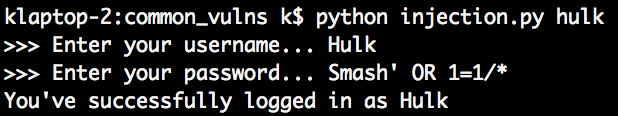
\includegraphics[scale=0.6]{inject}
\item
\item SQL injections can be prevented by using prepared statements, which create a sort of templated query. Input values are substituted separately using a separate protocol which does not require escaping characters like in a raw SQL query. This makes it resiliant against malicious user input, since that input is never interpreted as part of the query and used only as a parameter. SQL injections attacks remain pervasive because developers remain lax with their input sanitation. However methods to prevent malicious or malformed input from disrupting SQL queries do exist and when used provide a reliable safeguard against such injections.\\

In python, never use:
\begin{python}
cur.execute("""SELECT 1 FROM Users
    WHERE username = '%s' 
    AND password = '%s'""" 
    % (username, password))
\end{python}
Instead, use:
\begin{python}
cur.execute("""SELECT 1 FROM Users
    WHERE username = '%s' 
    AND password = '%s'""" ,
    (username, password))
\end{python}

This makes the SQL injection incur an error:\\
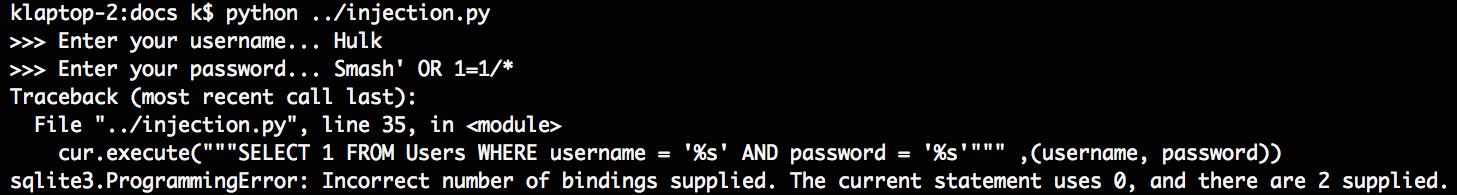
\includegraphics[scale=0.6]{inject_fixed}

\end{enumerate}

\end{document}
